\documentclass[12pt]{article}
\usepackage{sectsty}
\usepackage{titling}
\sectionfont{\small}
\subsectionfont{\small}
%\subsubsectionfont{\large}
%\paragraphfont{\large}
\usepackage{caption}
\usepackage{graphicx}
\usepackage{hyperref}
\usepackage{authblk}
\usepackage{titling}
\usepackage{multicol}
\hypersetup{
	colorlinks,
	citecolor=black,
	filecolor=black,
	linkcolor=black,
	urlcolor=blue
}
\usepackage{refstyle}
\usepackage{lipsum}
\usepackage{float}
\usepackage[table]{xcolor}
\usepackage{multirow}
\usepackage[letterpaper, margin=1.25in]{geometry}

%	\%



%	

\begin{document}
		

	
	
	
	\begin{center}
		\title*{\Huge June 24 BBQ:\\ 4545 Center Blvd, LIC, NY 10011}
	\end{center}
		
		\begin{figure}[H]
			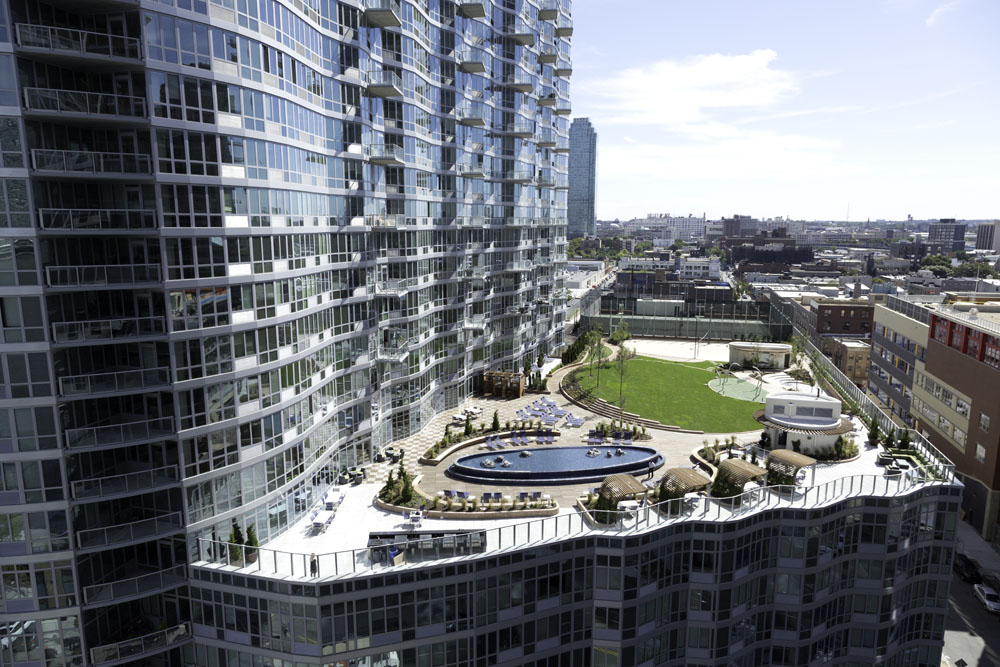
\includegraphics[width=\linewidth]{1}
		\end{figure}	
	\date{}

	
	
\section*{Introduction}
	This document is used as a tentative plan for planning BBQ at 4545 Center Blvd, LIC, NY 10011 on June 24, 2017. This document is separated into the following sections:
	\begin{itemize}
		\item Food needed		
		\item Food related materials needed
		\item Misc
		\item Tentative plan for getting above items
	\end{itemize}
	


\section*{Food Needed}
	Currently 11(or 12) people are invited, including 8 male and 3 female. Thus a target of food is around 70\% meat and 30\% non-meat
	
	
	Meat:
	\\
	\begin{center}
	\begin{tabular}{|c|c|}
		\hline
		        Meat          & lbs \\ \hline
		        Pork          &  2  \\ \hline
		        Beef          &  2  \\ \hline
		    Chicken wings     &  2  \\ \hline
		  Chicken drumstick   &  2  \\ \hline
			 Fish	&  2  \\ \hline
		Sausage (long / flat) &  2  \\ \hline
		        Ribs          &  2  \\ \hline
	\end{tabular} 
		\end{center}
	
	Non-meat:
	
	\begin{center}
	\begin{tabular}{|c|c|}
		\hline
		 Mushroom  & 1 bag \\ \hline
		  Pepper   & 1 bag \\ \hline
		   Corn    & 1 bag \\ \hline
		Califlower &   1   \\ \hline
		  Potato   &   2   \\ \hline
		  Onion    &   2   \\ \hline
	\end{tabular} 	
	\end{center}
	
	Drinks: 
	
	\begin{center}
		\begin{tabular}{|c|c|}
			\hline
			 Soda(Coke)  & 1-2 Bottle(1.5L) \\ \hline
			Soda(Sprite) & 1-2 Bottle(1.5L) \\ \hline
			    Beer     &    12 Bottle     \\ \hline
			   Water     & 2-3 Bottle(1.5L) \\ \hline
		\end{tabular} 	
	\end{center}	
	
	
\section*{Food related materials Needed}
	Various items are summarized in table below.
	\begin{center}

		\begin{tabular}{|c|}
			\hline
			                  Ketchup                   \\ \hline
			                Mayonnaise                  \\ \hline
			        Crackers  chips/tortillas)          \\ \hline
			                   Apron                    \\ \hline
			               Aluminum Foil                \\ \hline
			                  Napkins                   \\ \hline
			               Bottle Opener                \\ \hline
			               Fork \& knife                \\ \hline
			BBQ tool set (Steel Spatula, Locking Tongs) \\ \hline
			                   Cups                     \\ \hline
		\end{tabular} 
		\end{center}
	

\section*{Misc}
	

	Feel free to add in any food you wish to bring.

\section*{Getting above items}
	Fill in food you wish to take care of. 
	


\end{document}